\section{Counting Sort}
\label{sec:algorithm}

Counting sort, like radix sort, relies on array indexing rather than
comparison to order elements. The key idea of counting sort is to
count the number of occurrences of each element, and then perform a
prefix sum over all the counts. The prefix sum generates an array
which, for each element in the original array, will point to its
position in the final sorted array. In order for this to work,
counting sort needs a lower and upper bound on the values of the
elements in the input array. Counting sort is typically explained in
terms of sorting integers and we will do the same here.

The array \verb!{5,2,5,7,1}! will be used as a running example. In
addition, the range \verb!(1,10)! will be the approximation of the
range of the keys in the input. A diagrammatic illustration of our
running example is presented in figure \ref{fig:example}.

\begin{figure}
\begin{small} 
\begin{verbatim}
countingSort :: (Int,Int) 
                -> Array Int Int 
                -> Array Int Int
countingSort range input =
  reconstruct $
  scanlArray (+) 0 $
  histogram range input

histogram :: (Int,Int) 
             -> Array Int Int 
             -> Array Int Int
histogram range = 
  accumArray (\i _ -> i+1) 0 range . elems . fmap dup

reconstruct :: Array Int Int -> Array Int Int
reconstruct arr = 
  array (0,arr!l-1)
    [ (a,i)
    | (i,e) <- init (assocs arr)
    , a <- [ e .. arr!(i+1) - 1] ]
  where (_,l) = bounds arr

dup a = (a,a)
\end{verbatim}
\end{small}
\caption{A Haskell specification of Counting Sort. The function
  \texttt{scanlArray} is not standard but works much like
  \texttt{scanl}
  for lists.}
\label{fig:haskell}
\end{figure}

%% \begin{figure}
%% \begin{center}
%% 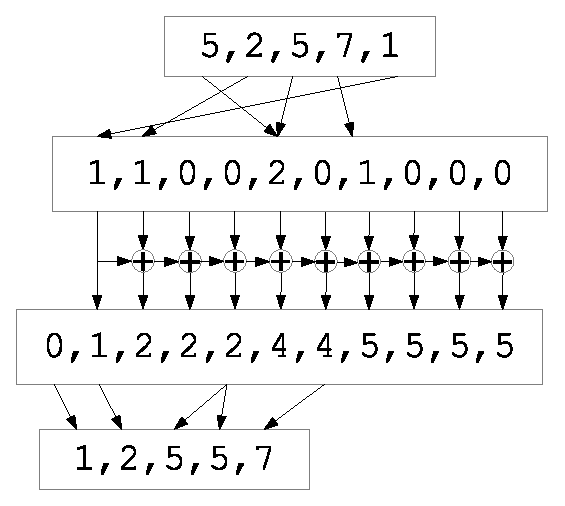
\includegraphics[height=4cm]{./CountingSortDiagram}
%% \end{center}
%% \caption{An example run of counting sort in diagrammatic form}
%% \label{fig:example}
%% \end{figure}
\begin{figure}

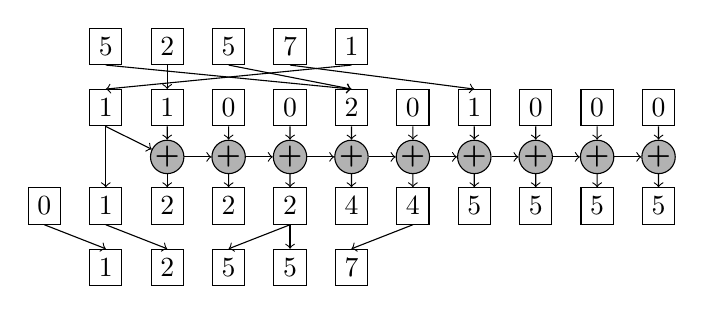
\begin{tikzpicture}[scale=0.78]
\usetikzlibrary{calc}
\tikzstyle{myedgestyle} = [->]
\tikzstyle{every node} = [draw, shape = rectangle]
 		 
\pgfmathsetmacro{\inpY}{1.5};
\pgfmathsetmacro{\vY}{\inpY-1};
\pgfmathsetmacro{\aY}{\vY-0.8};
\pgfmathsetmacro{\rY}{\aY-0.8};
\pgfmathsetmacro{\oY}{\rY-1};

\node (i0) at (1,\inpY) {$5$};
\node (i1) at (2,\inpY) {$2$};
\node (i2) at (3,\inpY) {$5$};
\node (i3) at (4,\inpY) {$7$};
\node (i4) at (5,\inpY) {$1$};

\node (v0) at (1,\vY) {$1$};
\node (v1) at (2,\vY) {$1$};
\node (v2) at (3,\vY) {$0$};
\node (v3) at (4,\vY) {$0$};
\node (v4) at (5,\vY) {$2$};
\node (v5) at (6,\vY) {$0$};
\node (v6) at (7,\vY) {$1$};
\node (v7) at (8,\vY) {$0$};
\node (v8) at (9,\vY) {$0$};
\node (v9) at (10,\vY) {$0$};

\draw [->] (i0.south) -- (v4.north);
\draw [->] (i1.south) -- (v1.north);
\draw [->] (i2.south) -- (v4.north);
\draw [->] (i3.south) -- (v6.north);
\draw [->] (i4.south) -- (v0.north);

\node (re) at (0,\rY) {$0$};
\node (r0) at (1,\rY) {$1$};
\node (r1) at (2,\rY) {$2$};
\node (r2) at (3,\rY) {$2$};
\node (r3) at (4,\rY) {$2$};
\node (r4) at (5,\rY) {$4$};
\node (r5) at (6,\rY) {$4$};
\node (r6) at (7,\rY) {$5$};
\node (r7) at (8,\rY) {$5$};
\node (r8) at (9,\rY) {$5$};
\node (r9) at (10,\rY) {$5$};


\tikzstyle{every node} = [draw, inner sep=0.1, fill=gray!60,shape = circle]

\node (1) at (2,\aY) {\bf{+}};
\node (2) at (3,\aY) {\bf{+}};
\node (3) at (4,\aY) {\bf{+}};
\node (4) at (5,\aY) {\bf{+}};
\node (5) at (6,\aY) {\bf{+}};
\node (6) at (7,\aY) {\bf{+}};
\node (7) at (8,\aY) {\bf{+}};
\node (8) at (9,\aY) {\bf{+}};
\node (9) at (10,\aY) {\bf{+}};


\foreach \i in {1,...,9}
{
	\draw [->] (v\i.south) -- (\i);
	\draw [->] (\i.south) -- (r\i);
}

\foreach \i in {1,...,8}
{
    \pgfmathtruncatemacro{\n}{(\i+1)};
    \draw [->] (\i) -- (\n);
}

\draw [->] (v0.south) -- (r0);
\draw [->] (v0.south) -- (1);

\tikzstyle{every node} = [draw, shape = rectangle]
\node (o0) at (1,\oY) {$1$};
\node (o1) at (2,\oY) {$2$};
\node (o2) at (3,\oY) {$5$};
\node (o3) at (4,\oY) {$5$};
\node (o4) at (5,\oY) {$7$};

\draw [->] (re.south) -- (o0.north);
\draw [->] (r0.south) -- (o1.north);
\draw [->] (r3.south) -- (o2.north);
\draw [->] (r3.south) -- (o3.north);
\draw [->] (r5.south) -- (o4.north);

\end{tikzpicture}

\caption{An example run of counting sort in diagrammatic form}
\label{fig:example}
\end{figure}
 
Counting sort consists of three steps: histogram creation, prefix sum
and reconstruction.

The histogram creation step computes a new array which records how
many times an integer occurs in the input array, i.e. the new array is
a histogram of the input array. The size and indices of the histogram
array are determined by the range which approximates the lower and
upper bounds of the keys.

Computing the histogram of \verb!{5,2,5,7,1}! with the range \verb!(1,10)!, 
results in \verb!{1,1,0,0,2,0,1,0,0,0}!.
%When running the example array \verb!{5,2,5,7,1}! through \\
%\verb!histogram! together with the range \verb!(1,10)! the resulting
%histogram is \verb!{1,1,0,0,2,0,1,0,0,0}!. 
Indexing in this array
starts at \verb!1! because that's the lower bound given in the
range. Each element in the histogram indicates how many times the
corresponding value occurs in the input array. For example, \verb!5!
occurs twice and \verb!8! occurs zero times.

The second step of the algorithm computes the prefix sum (or inclusive
scan with plus) of the histogram array, and prepends a zero.  For input array
\verb!{5,2,5,7,1}!  and range \verb!(1,10)!, the histogram array is
\verb!{1,1,0,0,2,0,1,0,0,0}! and its prefix sum is {\tt
  \{0,1,2,2,2,4,\allowbreak{}4,5,5,5,5\}}. 

%\verb!{0,1,2,2,2,4,4,5,5,5,5}!. This array starts with 0 and is one
%longer than the histogram array.

The array computed by the prefix sum is called the position array. It
indicates where in the final sorted array each value is placed. The
indices of the position array correspond to values in the final array
and the elements correspond to positions in the final array. The
reconstruct step takes care of distributing the values into the final
sorted array. For each index in the position array, the difference
between the element at that index and the index plus one is
computed. This difference indicates how many times the value occurs in
the final array.

The position array in our running example is {\tt\{0,1,2,2,2,4,\allowbreak{}4,5,5,5,5\}}.
Indexing starts at \verb!1! just as with the histogram. As an example,
element \verb!1! occurs once in the final array because the
difference between the element at position \verb!1! and \verb!2! in
the position array is precisely one. Also, \verb!1! is placed
on index \verb!0!. Furthermore, element \verb!5! occurs twice in
the final array (the difference between \verb!2! and \verb!4! in the
position array), on indices \verb!2! and \verb!3!. Continuing this
process with all elements will result in the following final array:
\verb!{1,2,5,5,7}!.

A functional description of counting sort can be found in figure
\ref{fig:haskell}. The main function is \verb!countingSort! which
takes two arguments: a range with a safe approximation of the lower
and upper bounds of the values in the input array, and the input array
itself. The histogram step is implemented by the function
\verb!histogram!, the prefix sum with \verb!scanlArray! and the
reconstruct step with the function \verb!reconstruct!.

\subsection{Occurrence sort: Removing duplicates}

There is an interesting variation of counting sort which removes
duplicate elements. It seems to be folklore; it is mentioned on
Wikipedia \cite{wikipedia}. However, we haven't found any description
of it in the literature. It is particularly interesting because it
allows for an efficient data-parallel implementation.
%% something which
%% will be explored in section \ref{sec:parallel}. Here we focus on the 
%% functional specification of the algorithm.
%% The rest of this
%% section will focus on the functional specification of the algorithm.


\begin{figure}
\begin{small}
\begin{verbatim}
countingSort :: (Int,Int) 
                -> Array Int Int 
                -> Array Int Int
countingSort range input =
  reconstruct $
  scanlArray (+) 0 $
  occurs range input

occurs :: (Int,Int) 
          -> Array Int Int 
          -> Array Int Int
occurs range = 
  accumArray (\_ _ -> 1) 0 range . elems . fmap dup
\end{verbatim}
\end{small}
\caption{A Haskell specification of occurrence sort}
\label{fig:duphaskell}
\end{figure}

Figure \ref{fig:duphaskell} shows the changes we make 
to counting sort in order to obtain occurrence sort.
%% counting sort compute a sorted array and at the same time remove
%% duplicate elements. 
Only the \verb!histogram! function needs changing
so that instead of computing an actual histogram which counts the
number of occurrences of an element, it only records if an element
occurs or not with a \verb!1! or a \verb!0!. Since the function
no longer computes a histogram it has been renamed to
\verb!occurs!.

The prefix sum and the reconstruction step can be kept intact. They
will still compute the correct result.

Compared to the full counting sort, occurrence sort has some
interesting properties which make it more suited for parallel execution.
In particular, the histogram construction phase and the reconstruction
phase allow for less synchronisation.

When constructing the histogram in the counting sort algorithm, an
index has to be incremented each time the corresponding value is found
in the input array. When parallelising this operation, it is important
that the increments are done atomically, which incurs a cost. The occurs
phase presented above doesn't need to employ any special mechanism to
ensure atomicity, since it writes a single word with the value $1$ to
memory.

Given the array \verb!{5,2,5,7,1}! as input and \verb!(1,10)!  as
range, the occurs step will now compute
\verb!{1,1,0,0,1,0,1,0,0,0}!. The prefix sum will in turn produce the
following position array: \verb!{0,1,2,2,2,3,3,4,4,4,4}!. The
reconstruct step computes \verb!{1,2,5,7}!. In particular,
there is only one occurrence of \verb!5! in the final array.
